\section{Auswertung}

\subsection{Nulleffekt}

Vor der Messung von den Halbwertszeiten muss der Nulleffekt bestimmt werden. Dabei
wird über ein Intervall von $\Delta t = \SI{800}{\second}$ die Zählrate des Zählrohrs
gemessen ohne eine Radioaktive Substanz. Es wurden $N_{\Delta t , U} = 200$ gemessen.
Auf eine Sekunde umgerechnet ergibt das eine Zählrate von:

\begin{equation*}
  N_U = \SI{0.250(18)}{\per\second}
\end{equation*}

\subsection{Indium}

Zunächst wird die Zerfallskurve von Indium gemessen. Für Indium wird ein Zeitintervall
von $\Delta t = \SI{240}{\second}$ gewählt. Damit ergibt sich für den Nulleffekt
$N_U = \num{60.00(424)}$. Der Nulleffekt muss von jedem Messwert abgezogen werden.
Die Messwerte sind in der Tabelle \ref{tab:1} dargestellt.

\begin{table}[H]
  \centering
  \caption{Messaufnahme von Indium (In).}
  \label{tab:1}
  \begin{tabular}{c c c c}
    \toprule
    $t \, /\, s$& $N_{\Delta t}$& $t \, /\, s$& $N_{\Delta t}$ \\
    \midrule
    240  &  2930 & 2160 & 1773\\
    480  &  2710 & 2400 & 1710\\
    720  &  2604 & 2640 & 1710\\
    960  &  2258 & 2880 & 1543\\
    1200 &  2229 & 3120 & 1514\\
    1440 &  2117 & 3360 & 1446\\
    1680 &  1900 & 3600 & 1436\\
    1920 &  1923 & - & -\\
    \bottomrule
  \end{tabular}
\end{table}

Um nun aus den Messwerten die Halbwertszeit von Indium zu bestimmen werden die
Messwerte in einem halblogarithmischen Diagramm dargestellt, in der Abbildung \ref{abb:3}.
Nun lässt sich eine lineare Ausgleichsrechnung durchführen, da die Gleichung
\ref{eq:3} durch das Logarithmieren zu der folgenden Gleichung wird:

\begin{equation}
  \ln(N_{\Delta t}(t)) = -\lambda t + \ln(N_0(1-e^{-\lambda \Delta t}) = - m \cdot t + b.
  \label{eq:4}
\end{equation}

\begin{figure}[H]
  \centering
  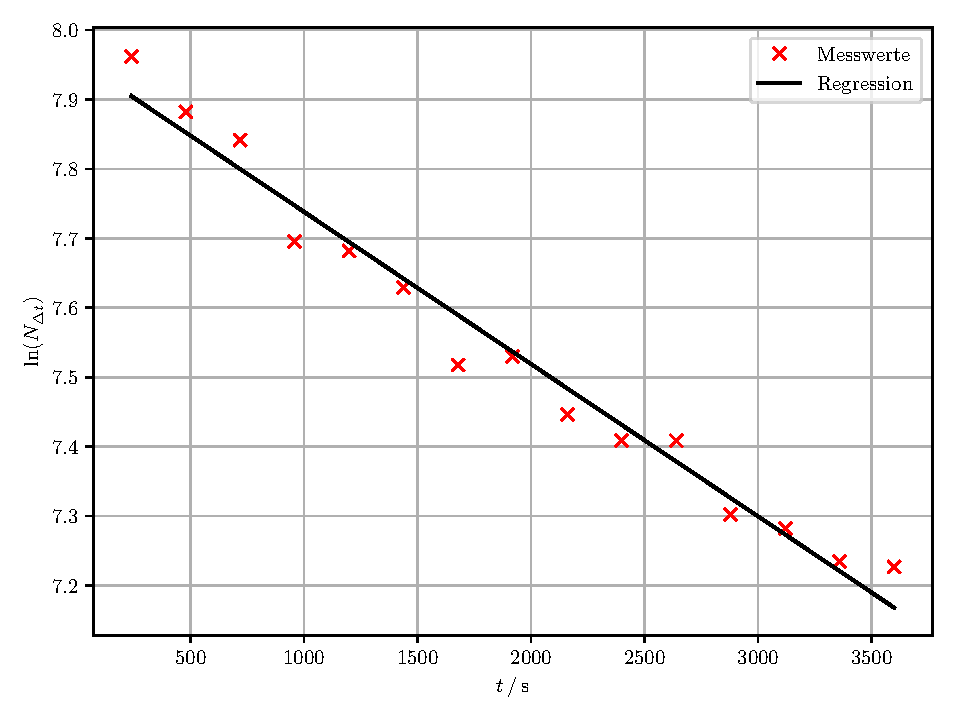
\includegraphics{plot3.pdf}
  \caption{Darstellung der Logarithmierten Messwerte von Indium und die Ausgleichsrechnung.}
  \label{abb:3}
\end{figure}

Die Ausgleichsrechnung wird mit Python 3.6 durchgeführt. Durch die Subtraktion der
Messwerte mit den fehlerbehafteten Nulleffekt hat jeder Messwert einen Fehler, welcher
durch das Logarithmieren allerdings so klein wird, dass sie in dem Graphen nicht
durch Fehlerbalken darstellbar sind. Der Fehler lässt sich mit folgender Gleichung
bestimmen:

\begin{equation*}
  \Delta \ln(N(t)) = \sqrt{\left( \frac{1}{N(t)}\right)^2 \cdot \Delta N(t)^2}
\end{equation*}

Durch die Ausgleichsrechnung ergibt sich für die Parameter der Geraden:

\begin{itemize}
  \item m = \SI{21.932(1006)e-5}{\per\second}
  \item b = \num{7.958(22)}
\end{itemize}

Mit der Gleichung \ref{eq:2} lässt sich nun aus $m = \lambda$ die Halbwertzeit bestimmen.
Da mit fehlerbehafteten Größen gerechnet wird, wird der Fehler mithilfe der Gauß´schen
Fehlerfortpflanzung bestimmt:

\begin{equation*}
  \Delta T = \sqrt{\left(-\frac{\ln(2)}{\lambda^2}\right)^2 \cdot (\Delta \lambda)^2}
\end{equation*}

Damit ergibt sich für die Halbwertszeit von Indium:

\begin{equation*}
  T_{In} = \SI{3160(140)}{\second}
\end{equation*}

Nun soll noch die Größe von $N(0)(1-e^{-\lambda \Delta t}) = e^b$ bestimmt werden.
Auch für diese Rechnung wird die Fehlerfortpflanzung verwendet. Sie ergibt sich zu:

\begin{equation*}
  \Delta (e^b) = \sqrt{\left( b e^b\right)^2 \cdot (\Delta b)^2}
\end{equation*}

Damit folgt für den Term:

\begin{equation*}
  N(0)(1-e^{-\lambda \Delta t}) = \num{2860(60)}
\end{equation*}


\subsection{Silber}
Auch von den Silbermesswerten muss der Nulleffekt abgezogen werden. Das Zeitintervall
war bei dieser Messreihe $\Delta t = \SI{10}{\second}$, deshalb folgt für den Nulleffekt
$N_U = \num{2.500(176)}$.
Die Messwerte sind in der Tabelle \ref{tab:2} dargestellt und werden für die Ausgleichsrechnung
wie bei Indium Logarithmiert.
Die Messwerte haben durch den Nulleffekt wieder einen
statistischen Fehler. Da die Messwerte allerdings für die Ausgleichsrechnung wieder
Logarithmiert werden, werden die Fehler bei den meisten Messwerten so klein,
dass die Fehlerbalken bei dem Graphen nicht sichtbar sind.

\begin{table}[H]
  \centering
  \caption{Messaufnahme von Silber (Ag).}
  \label{tab:2}
  \begin{tabular}{c c c c c c c c}
    \toprule
    $t \, /\, s$& $N_{\Delta t}$& $t \, /\, s$& $N_{\Delta t}$ & $t \, /\, s$& $N_{\Delta t}$ & $t \, /\, s$& $N_{\Delta t}$ \\
    \midrule
    10 & 387 & 130 & 25 & 250 & 10 & 370 & 8\\
    20 & 143 & 140 & 25 & 260 & 14 & 380 & 5\\
    30 & 113 & 150 & 30 & 270 & 20 & 390 & 11\\
    40 & 116 & 160 & 27 & 280 & 13 & 400 & 8\\
    50 & 82 & 170 & 13 & 290 & 10 & 410 & \cellcolor{red}2\\
    60 & 58 & 180 & 27 & 300 & 30 & 420 & 11\\
    70 & 60 & 190 & 18 & 310 & 10 & -&-\\
    80 & 45 & 200 & 21 & 320 & 9 & -& - \\
    90 & 51 & 210 & 17 & 330 & 10 & -& -\\
    100 & 36 & 220 & 10 & 340 & 15 &- &-\\
    110 & 33 & 230 & 22 & 350 & 10 &- &-\\
    120 & 31 & 240 & 14 & 360 & 12 &- &-\\
    \bottomrule
  \end{tabular}
\end{table}

Der markierte Messwert wurde aus dem Graphen herausgenommen, da er negativ wird
nachdem der Nulleffekt abgezogen wird.
Da reines Silber aus den Isotopen $^108Ag$ und $^110Ag$ besteht, finden zwei Zerfälle
gleichzeitig statt. Das bedeutet, dass zwei Ausgleichsrechnungen
durchgeführt werden müssen, für den kurzlebigen Zerfall und den langlebigen.
Die Messwerte und Ausgleichsrechnungen sind in der Abbildung \ref{abb:4} dargestellt.

\begin{figure}[H]
  \centering
  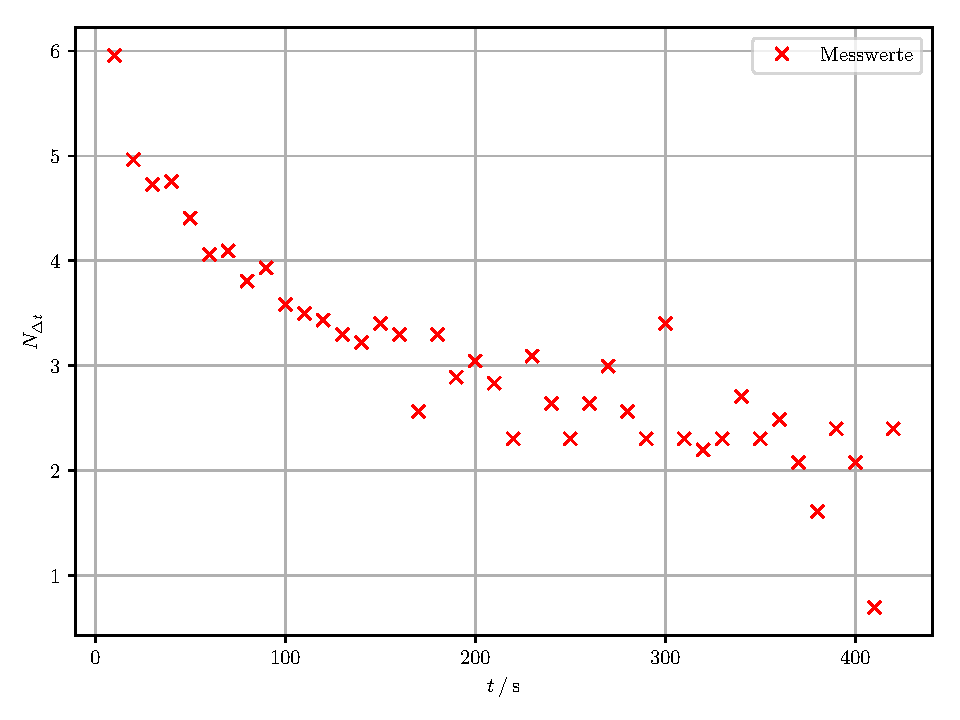
\includegraphics{plot1.pdf}
  \caption{Darstellung der Messwerte für den gesamten Zerfall und die errechneten Werte
  für den kurzlebigen Zerfall.}
  \label{abb:4}
\end{figure}

Zur Berechnung des langlebigen Zerfalls wird eine Zeit festgelegt, ab welcher die
logarithmierten Messwerte näherungweise linear sind. Diese Zeit war in diesem Fall
$t^* = \SI{250}{\second}$. Ab diesem Punkt wird nun wieder eine lineare Ausgleichsrechnung
mit Python 3.6 durchgeführt, wobei die Geradengleichung wieder Gleichung \ref{eq:4}
ist. Damit ergibt sich für die Parameter der Geraden:

\begin{itemize}
  \item m = \SI{4.575(2287)e-3}{\per\second}
  \item b = \num{3.648(765)}
\end{itemize}

Nun lässt sich aus m die Halbwertzeit für diesen Zerfall bestimmen. Die Berechnung
des Fehlers ist auch analog zu Indium.

\begin{equation*}
  T_\text{lang} = \SI{150(80)}{\second}
\end{equation*}

Mithilfe der Gleichung für die Ausgleichsgerade lässt sich eine Gleichung für
$N_\text{lang}(t)$ herleiten. Dabei muss die Exponentialfunktion auf die Gleichung
angewendet werden. Der Fehler von $N_\text{lang}(t)$ lässt sich mit folgender
Formel bestimmen:

\begin{equation*}
  \Delta N_\text{lang}(t) = \sqrt{\left(-te^{-mt+b}\right)^2 \cdot (\Delta m)^2 +
  \left(e^{-mt+b}\right)^2 \cdot (\Delta b)^2}
\end{equation*}

Von der gesamt gemessenen Zählrate muss nun $\Delta N_\text{lang}(t_i)$ abgezogen
werden, also

\begin{equation*}
\Delta N_\text{kurz}(t_i) = \Delta N_\text{ges}(t_i) - \Delta N_\text{lang}(t_i).
\end{equation*}

Das Zeitintervall $t_i$ muss so gewählt werden, dass $\Delta N_\text{kurz}(t_i)$
positiv ist, weil sonst eine Auswertung unmöglich ist. In diesem Fall ist das
Intervall vom Anfang der Messung bis $t = \SI{120}{\second}$.
Zuletzt werden die errechneten Messwerte wieder logarithmiert, um eine lineare
Ausgleichsrechnung durchführen zu können. Diese Werte und die Ausgleichsgerade sind
auch in Abbildung \ref{abb:4} dargestellt. Die Ausgleichsrechnung wird wieder mit
Python 3.6 durchgeführt und die Parameter der Geradengleichung entsprechen wieder der
Gleichung \ref{eq:4}. Damit ergeben sich die Parameter:

\begin{itemize}
  \item m = \SI{3.236(260)e-2}{\per\second}
  \item b = \num{5.584(192)}
\end{itemize}

Aus diesen Parametern lässt sich nun auch wieder die Halbwertzeit für den kurzlebigen
Zerfall bestimmen. Die Rechnung ist analog wie bei Indium.

\begin{equation*}
  T_\text{kurz} = \SI{21.4(17)}{\second}
\end{equation*}

Als letztes wird noch eine Summenkurve aus den zwei bestimmten Zerfallsgeraden bestimmt.
Dazu wird auf die Ausgleichsgeraden die Exponentialfunktion angewendet um wieder einen
Ausdruck für $N_\text{kurz}(t)$ und $N_\text{lang}(t)$ zu erhalten. Dann werden die
Funktionen addiert. Die Summenkurve und die Messwerte sind in Abbildung \ref{abb:5}
dargestellt.

\begin{figure}[H]
  \centering
  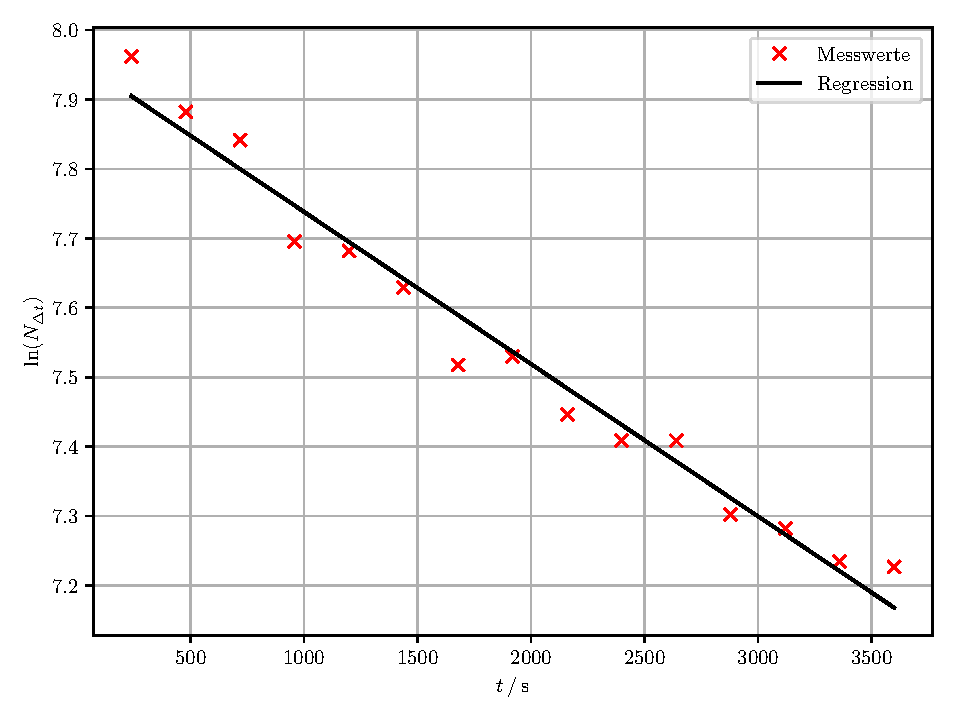
\includegraphics{plot2.pdf}
  \caption{Darstellung der Messwerte und der Summenkurve.}
  \label{abb:5}
\end{figure}
